\documentclass{mproj}
\usepackage{graphicx}

\usepackage{url}
\usepackage{fancyvrb}
\usepackage[final]{pdfpages}
\usepackage{times}

% for alternative page numbering use the following package
% and see documentation for commands
%\usepackage{fancyheadings}


% other potentially useful packages
%\uspackage{amssymb,amsmath}
%\usepackage{url}
%\usepackage{fancyvrb}
%\usepackage[final]{pdfpages}

\begin{document}
%%%%%%%%%%%%%%%%%%%%%%%%%%%%%%%%%%%%%%%%%%%%%%%%%%%%%%%%%%%%%%%%%%%
\title{Title of project placed here}
\author{Name of author placed here}
\date{Date of submission placed here}
\maketitle
%%%%%%%%%%%%%%%%%%%%%%%%%%%%%%%%%%%%%%%%%%%%%%%%%%%%%%%%%%%%%%%%%%%

%%%%%%%%%%%%%%%%%%%%%%%%%%%%%%%%%%%%%%%%%%%%%%%%%%%%%%%%%%%%%%%%%%%
\begin{abstract}
abstract goes here
\end{abstract}
%%%%%%%%%%%%%%%%%%%%%%%%%%%%%%%%%%%%%%%%%%%%%%%%%%%%%%%%%%%%%%%%%%%

%%%%%%%%%%%%%%%%%%%%%%%%%%%%%%%%%%%%%%%%%%%%%%%%%%%%%%%%%%%%%%%%%%%
\educationalconsent

%%%%%%%%%%%%%%%%%%%%%%%%%%%%%%%%%%%%%%%%%%%%%%%%%%%%%%%%%%%%%%%%%%%

\newpage
%%%%%%%%%%%%%%%%%%%%%%%%%%%%%%%%%%%%%%%%%%%%%%%%%%%%%%%%%%%%%%%%%%%
\section*{Acknowledgements}

acknowledgements go here sdfsdf

%%%%%%%%%%%%%%%%%%%%%%%%%%%%%%%%%%%%%%%%%%%%%%%%%%%%%%%%%%%%%%%%%%%
\tableofcontents
%%%%%%%%%%%%%%%%%%%%%%%%%%%%%%%%%%%%%%%%%%%%%%%%%%%%%%%%%%%%%%%%%%%

%%%%%%%%%%%%%%%%%%%%%%%%%%%%%%%%%%%%%%%%%%%%%%%%%%%%%%%%%%%%%%%%%%%
\chapter{Introduction}\label{intro}

\section{Sentence}

I completed a program which allowed a turtlebot to autonomously map an environment using SLAM as well as create an inventory of items found in the environment.


\section{Importance/Context/Motivation}

Mobile robots are becoming more and more affordable and accessible which has allowed developers to take advantage of their applications in many different ways. 

SLAM has it's application in rescue robots which
http://www.aaai.org/Pressroom/Releases/release-02-0910.php
these robots required realtime control and utilised only video streams to identify and rescue people.

This compares to this which utilises rugged mobile robots to create SLAM maps of mine shafts with minimal supersvision. This can then be applied to areas which are too unsafe/ small for humans to access.
https://miningrox.informatik.tu-freiberg.de/en/

More affordable Drones can also be used to increasingly accurate create maps of property as well

Object detection can be used to detect humans via heat sensors etc. Aswell as identifying bombs etc.



\section{Objectives/Hypothesis Karl Popper/Problem statement}

\section{Description of Objectives}

\section{How I achieved it} 

\subsection{System Diagram} 

\section{Outline of the dissertation} 




%%%%%%%%%%%%%%%%%%%%%%%%%%%%%%%%%%%%%%%%%%%%%%%%%%%%%%%%%%%%%%%%%%%
\chapter{Background}\label{survey}

Existing/similar applications

Why choosing to talk about these things. 

More references.

Include Photos of everything
\section{Papers}
Semantic Slam
\section{Robot Operating System (ROS)}
\subsection{What is ROS}

ROS is a meta-operating system which provides a collection of tools and conventions to aid the writing of robot software. This includes an abstraction of hardware and communications as well as tools including message passing, package management and low level controllers.

\subsection{Why do people use ROS}

ROS features open-source licenses and a large growing collection of packages which contribute to a vibrant ecosystem of developers and researchers working on applications. Some of these packages includes powerful applications such as the Gazebo simulator and the visualisation tool RViz as well as complex algorithms such as SLAM and drivers such as OpenNI.

ROS encourages software engineering principles of loose coupling and abstraction which simplifies software integration and reuse as well as meaning that ROS is generally independent of hardware specifics. ROS features standard implementations in popular programming languages such as Python and C++ which increases adoption.

\subsection{How does ROS works?}

ROS consists of some key components within the communications infrastructure.
\begin{itemize}
  \item Nodes are modular processes performing computation which can communicate with each other using topics or services. A system may consist of many nodes which perform many different tasks.
  \item Topics are named buses which provide a clear message passing interface between nodes. This is achieved through an anonymous publish/subscribe mechanism. This mechanism allows many-to-many transport.
  \item Messages are a data structure which are published by nodes to topics. They support strongly typed fields such as primitives or arrays and are either predefined or user-defined.
  \item The ROS core or Master provides a centralized node which locates and negotiates communications between nodes as well providing naming and registration services.
  \item Services forgo the many-to-many paradigm and provide a request/reply interaction via servers and clients.

\end{itemize}

\begin{figure}[h]
  \caption{Illustration of the ROS concepts}
  \centering
  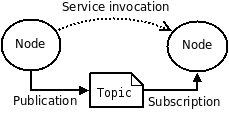
\includegraphics[width=0.5\textwidth]{images/ROS_basic_concepts.png}
  \label{fig:ROS diagram}
\end{figure}

For example a simple robot vehicle system can consist of three nodes. The first node controls the robot's ultrasonic range finder and is publishing a stream of range messages taken from the sensor along the \texttt{sensor/sonar} topic.

The second node controls the robot's movement hardware and is publishing the robot's orientation on the \texttt{geometry\char`_msgs/pose} topic. It also contains an actionlib server which responses to requests to change the robot's positioning. 

The third node controls the robot's movement and is subscribed to the \texttt{sensor/sonar} topic and contains a client of the actionlib server. While processing the range messages if the range indicated is very small the node can use the actionlib service to request an adjustment in the orientation of the robot thus meaning the robot will avoid collisions. 

Include diagram describing example


\subsubsection{RViz}

Rviz is a visualisation tool in ROS which provides 3d visualisations of sensor data and robot states, such as cameras, lasers and joint states. Add modular componets which can be customized.

\subsubsection{Gazebo}
Gazebo provides a simulated environment to build and test applications in ROS. A simulated robot will feature all the same sensors as a real one and a model world can be created. Physics, models, programmable features such as doors orlights.


\section{Mobile Robots}


Mobile robots are robots that are not fixed to one location and are capable of moving around their environments. Movement is achieved generally through legs, wheels or tracks but aerial and nautical robots can use propellors. The robot can be controlled through manual-tele operation involving a human driver, line-following which follow visual cues such as painted lines to navigate or autonomously.



These robots have many applications covering military, agricultural, rescue, transport and domestic usage.


 For example: Unmanned Ground Vehicles can include military robots but also self-driving cars and
delivery robots. Aerial robots (UAVs) , underwate(AUVS).

Drone missles, resucue robots, self driving cars, roomba, mail robots.

\subsection{Turtlebot 2}


The Turtlebot 2 is a part of a series of low cost, open-source mobile robots by Clearpath Robotics**. These robots are intended for educational and research purposes and provide an 'low-barrier-of-entry' platform for development. The robot consists of a Kobuki base, a computer running ROS and some form of RGB-D or Stereo Camera such as the Xbox Kinect or Asus Xtion.

The Kobuki Base contains IR, bump, cliff and wheel drop sensors as well as different power connectors and ports.

The Kobuki Base requires a computer running ROS to communicate with, in most cases this can simply involve a laptop attached to the top of the base connected by a usb cable. However in some cases it may be more convienent to attach a small netbook or Raspberry Pi to the base and use a seperate computer to communicate with the host.

- Lots of software standard packages support, gazebo models, teleoperation, slam as well as large and growing community of stuff...
- Abstracted hardware, no need to understand how it works, just recieve the data,

How it works in ros
Odometry
\section{Cameras}
Why do we need them
Why discuss both of these? - exemplar
\subsection{RGB-D}
\begin{itemize}
  \item How it works
  \item Active camera - range finder
  \item Kinect specs
\end{itemize}
\subsection{Stereo}

\begin{itemize}
  \item Passive camera, works well outdoors
  \item How depth is calculated
  \item How images are combined 
  \item About the zed cam - specs
\end{itemize}

\section{SLAM}
\begin{itemize}

  \item What is the problem, include references e.g. to correlation
  \item explain the proble
  \item solutions to the problem

 
\end{itemize}


SLAM is the problem of simultaneously localising (finding the pose and orientation) of a camera within it's surroundings at the same time as mapping the structure of the environment. This requires a robot or camera with the ability to produce odometry readings as well as camera with a range measurement device, either a range finder or found in a stereo camera. 

SLAM forms the basis of navigation in most mobile robots, meaning unknown environments can be explored and mapped without the need for technology such as GPS which becomes innaccurate within two metres or in interiors. It has applications in a range of manned and autonomous robots. This includes UAV's, underwater robots and domestic robots such automatic lawnmowers. SLAM is a key component in the development of self-driving cars These cars which are driven along routes while performing SLAM capturing location, feature and obstacle data. Once the map is completed it is processed and the cars are driven autonomously along these routes updating the map as necessary.



This is considered to be a solved problem in Computer Science and their are many different approaches for finding a solution. \cite{Hugh2006}



During the development of the SLAM problem researchers established the correlation between estimates of a robots location and the landmarks which consituate the map







Building maps once can work, but it can be distrupted by changes in the environment, e.g lighting 

We know the position of the landmarks
Localisation requires landmarks, estimate the location of these and estimate it's own pose relative to it. This can be inaccurate due to odometry or inaccurate readings, rely on each. 95% --> give gaussian estimate
GEt estimate of where the robot probably is, get it's location relative to landmarks

Cannot fully decouple localisation and mapping as map is needed for localisation and a pose estimate is needed for mapping

Areas which are missing. Passive.

Given: Robot's controls, Observations(laser scans)
Wanted: map of environment
Path of the robot.

Probablistic techniques, uncertainity of robots motions and observations... represent uncertnity typically in a Gaussian distribution, error can accumalate over time. Take the uncertanity into account.

Slam is difficult because both path and map are unknown, but they are correlated and depend on each other





On a high level SLAM is solved by using the environment to update the pose of the robot.  Using odometry as the sole measurement of localisation has an element of uncertainity due to extraneous factors such as wheels slipping on different environments meaning that a stated distance given by an odometry reading may be over or under estimated. Therefore laser scans or other forms of depth readings are used to correct the robot's position by extracting features from the surrounding environment. These are called landmarks and can be extracted by various methods such as Random Sampling Consensus (RANSAC) and provide a growing map of the enviroment. 


The robot estimates the location of it's own pose relative to these different landmarks which are all correlated together and increase with successive observations. \cite{Hugh1988}
  
The combined localisation and mapping estimates as a single estimation problem are convergent  
  
  Extended Kalman Filter is used to update where the robot presumes it is based on these landmarks and keeps track of the uncertainity of the robots position and the landmarks seen.
  
  When robot moves the uncertainity of the new position is updated.
  Landmarks are extracted and reobserved ones are used to update the robots position. New landmarks are added to the EKF. 
  
  ***Diagram. of sequence of reaffirmation.


Uncertanity is kept track of.



\subsection{RtabMap}

- intro RTAB-Map is a RGB-D graph based SLAM approach. What it is

- Loop closure technique. How it works

Online slam, seeks to recover only the most recent pose, not the entire path algorithm

\subsection{Others}

Compare rtabmap and other papers Cartographer

\section{Frontier Exploration}






\section{Object Detection}

At low levels of the evolutionary scale the eye acts as a type of goal detector rather than a camera. 

The information provided by past experience have a greater say on how a scene has been interpreted than immediate information provided by external organs.
The eye the brain the computer p208

However in contrast to simple organisms whose focus is on detection resulting in a sensitive and broad field of vision the programme must have the ability to classify which requires precise resolution when required.

Everything is seen for the first time.
Our sensory systems does not keep telling us things we already know as most important environmental information stays constant, this process is called adaption and happens not only at a retinal level but at higher levels in the brain.

What different types of neural structure are used to extract information from a visual signal

1) areas of high level of features
2) depth/closeness
3) shapes/edge detection - particularly light and dark

Not feasible to search for objects at all locations in a visual field
Partioning or perceptual organisation.

Law of proximity = Stimulus that are close together are percieved to be a group.

Geometric, Photometric modeling scene degmentation, naming+labeling,

Image matching:
correlation approach
 
feature matching approach
eges remain across two images of the same scene. 
relational matching approach

From page 281 --> talk about image labeling

Neurophysiologic studies have shown that, in humans, these two 
factors are the main responsible ones to drive attention. Bottom-up factors emanate from the scene and 
focus attention on regions whose features are sufficiently discriminative with respect to the features 
of their surroundings. On the other hand, top-down factors are derived from cognitive issues, such as 
knowledge about the current task.
http://www.prip.tuwien.ac.at/people/krw/more/papers/2012/Antunez2012a.pdf

\subsection{opencv}
\subsection{Feature Detection}
\subsection{Deep Learning}
\subsubsection{Tensorflow}
\subsubsection{Haar Cascades}
\subsubsection{Google Vision API}
\subsubsection{3D Detection}
\subsection{Summary and Discussion}
\subsubsection{What currently exists for completing the objectives}
\subsubsection{What are the Gaps, What do I have to do to fill the gaps}
\subsubsection{What methods are not appropriate to fill the gap}




%%%%%%%%%%%%%%%%%%%%%%%%%%%%%%%%%%%%%%%%%%%%%%%%%%%%%%%%%%%%%%%%%%%
\chapter{Approach/Implementation/System Implementation}
\section{Anaylsis the approaches}

What problems I encounted etc.

\section{Mapping}
\subsection{Transforming data}
\subsection{Calibration}
\section{Frontier Exploration}
\section{Object Detection and Recognition}
\subsection{Blob Detection} 
\subsection{Detecting Clusters - different methods}
\subsection{Creating Boxes}
\subsection{Tracking Boxes}
\subsection{Positioning Boxes in Map/Loop Closure}
\subsection{Recognising Objects}
\subsection{Publishing to Rviz/Rtabmap}
\section{The whole package - how to utilise}
%%%%%%%%%%%%%%%%%%%%%%%%%%%%%%%%%%%%%%%%%%%%%%%%%%%%%%%%%%%%%%%%%%%
\chapter{Evaluation}
\section{Testing}

%%%%%%%%%%%%%%%%%%%%%%%%%%%%%%%%%%%%%%%%%%%%%%%%%%%%%%%%%%%%%%%%%%%
\chapter{Conclusion}\label{conclusion}
\subsection{Future work}

\appendix % first appendix
%%%%%%%%%%%%%%%%%%%%%%%%%%%%%%%%%%%%%%%%%%%%%%%%%%%%%%%%%%%%%%%%%%%
\chapter{First appendix}

\section{Section of first appendix}

%%%%%%%%%%%%%%%%%%%%%%%%%%%%%%%%%%%%%%%%%%%%%%%%%%%%%%%%%%%%%%%%%%%
\chapter{Second appendix}

%%%%%%%%%%%%%%%%%%%%%%%%%%%%%%%%%%%%%%%%%%%%%%%%%%%%%%%%%%%%%%%%%%%
% it is fine to change the bibliography style if you want
\bibliographystyle{plain}
\bibliography{mproj}
\end{document}
